\documentclass[12pt]{article}  
% Эта строка — комментарий, она не будет показана в выходном файле  
\usepackage[left=1cm,right=1cm,
top=2cm,bottom=2cm,bindingoffset=0cm]{geometry}
\usepackage{ucs} 
\usepackage[utf8x]{inputenc} % Включаем поддержку UTF8  
\usepackage[russian]{babel}  % Включаем пакет для поддержки русского языка  
\usepackage{amsmath}
\usepackage{listings}
\usepackage{color}
\usepackage{tikz}
\usepackage{pgfplots}
\usepackage{graphicx}

\definecolor{mygreen}{rgb}{0,0.6,0}
\definecolor{mygray}{rgb}{0.5,0.5,0.5}
\definecolor{mymauve}{rgb}{0.58,0,0.82}
\title{Отчет по лабораторной работе 6 \\ 
	По предмету “Анализ алгоритмов” \\
	По теме “Конвейер”
}  
\date{2018}  
\author{Фирсова Дарья ИУ7-56}

\begin{document}  
	\maketitle  
	\newpage
	\section*{Введение}
	В лабораторной работе изучается параллельный алгоритм конвейера. Используются очереди и средства синхронизации потоков. Конвейер можно использовать, когда задачу можно разбить на части, при этом каждый поток выполняет свою часть. После выпоолнения очередной задачи, результат вычислений передается на следующую "ленту". \\
	\textbf{Цель лабораторной работы:} составить алгоритм конвейра, использовать общие очереди и мьютексы, записать работу поэтапно в файл. В конвейере использовать 3 уровня.\\
\newpage

\section{Аналитеская часть}
В данном разделе приведены алгоритмы умножения.
\subsection{Описание алгоритмов}
Конвейер состоит из трех уровней и трех очередей. На первом уровне элемент поступает из первой очереди, и создаются два других числа возведением исходного в 2 и 4 степень. Затем оба элемента поступают во вторую очередь. На втором уровне элемент забирается элемент из второй очереди, возводится в степень 6 и 8, поступает в 3 очередь. На третьем уровне к полученному элементу прибавляется число и "лента" завершает работу.
\newpage
\section{Конструкторская часть}
В данном разделе представлена схема конвейера.

\begin{figure}[ht!]
	\centering
	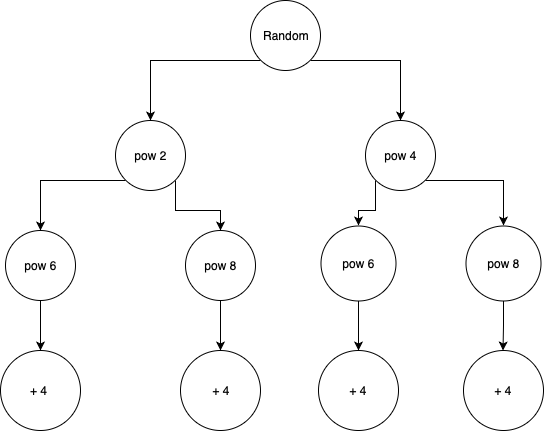
\includegraphics[width=180mm, height=150mm]{Diagram.png}
	\caption{Схема конвейра\label{overflow}}
\end{figure}
\newpage


\newpage
\newpage

\section{Технологическая часть}

В этом разделе приведена реализация функций, указан язык программирования и необходимые модули. 
\subsection{Средства реализации}
В данной работе использовался язык Python 3.6, в среде Pycharm. Для измерения времени использовался модуль time, измерения производились в секундах. Для создания потока использовался модуль threading. Для создания очередей модуль queue. 
\subsection{Листинг кода}
\lstset{ 
	backgroundcolor=\color{white},   % choose the background color; you must add \usepackage{color} or \usepackage{xcolor}; should come as last argument
	basicstyle=\footnotesize,        % the size of the fonts that are used for the code
	breakatwhitespace=false,         % sets if automatic breaks should only happen at whitespace
	breaklines=true,                 % sets automatic line breaking
	captionpos=b,                    % sets the caption-position to bottom
	commentstyle=\color{mygreen},    % comment style
	deletekeywords={...},            % if you want to delete keywords from the given language
	escapeinside={\%*}{*)},          % if you want to add LaTeX within your code
	extendedchars=true,              % lets you use non-ASCII characters; for 8-bits encodings only, does not work with UTF-8
	frame=single,	                   % adds a frame around the code
	keepspaces=true,                 % keeps spaces in text, useful for keeping indentation of code (possibly needs columns=flexible)
	keywordstyle=\color{blue},       % keyword style
	language=Python,                 % the language of the code
	morekeywords={*,...},            % if you want to add more keywords to the set
	numbers=left,                    % where to put the line-numbers; possible values are (none, left, right)
	numbersep=5pt,                   % how far the line-numbers are from the code
	numberstyle=\tiny\color{mygray}, % the style that is used for the line-numbers
	rulecolor=\color{black},         % if not set, the frame-color may be changed on line-breaks within not-black text (e.g. comments (green here))
	showspaces=false,                % show spaces everywhere adding particular underscores; it overrides 'showstringspaces'
	showstringspaces=false,          % underline spaces within strings only
	showtabs=false,                  % show tabs within strings adding particular underscores
	stepnumber=1,                    % the step between two line-numbers. If it's 1, each line will be numbered
	stringstyle=\color{mymauve},     % string literal style
	tabsize=1,	                   % sets default tabsize to 2 spaces
	title=Листинг 1. Реализация алгоритмов.                   % show the filename of files included with \lstinputlisting; also try caption instead of title
}
\lstinputlisting[language=Python]{mail.py}
\newpage

\newpage
\newpage

\section{Экспериментальная часть}
В данном разделе будут приведены примеры работы алгоритмов и произведены замеры времени. Тестирование производилось на компьютере с процессором Intel Core i5 (I5-6267U) и оперативной памятью 8 Гб. 
\subsection{Примеры работы}
Результат работы алгоритма находится в файле log.txt

\newpage
\subsection{Вывод}
В файле лога можно увидеть, что значения на каждом этапе вычисляются параллельно. 
На вход подаются 50 случайных значений, выходных значений в 4 раза больше. В результате работы программы вычисляются степени числа. 

\newpage
\section{Заключение}
В лабораторной работе разработаны алгоритмы параллельного вычисления для разработки конвейера. Были изучены механизмы работы очередей, мьютексов и потоков. Для составления отчета использован Latex.
\\
\end{document}